\documentclass[spanish, fleqn]{article}
\usepackage{babel}
\usepackage[utf8]{inputenc}
\usepackage{amsmath}
\usepackage{amsfonts}
\usepackage{wasysym}
\usepackage[colorlinks, urlcolor=blue]{hyperref}
\usepackage[top = 2.5cm, bottom = 2cm, left = 2cm, right = 2cm]{geometry}

\usepackage{pdflscape}
\usepackage{listings}
\usepackage{color}
\usepackage{tikz}
\usetikzlibrary{plotmarks}

\newcommand{\rojo}{\textcolor{red}}

\title{ILI 292 - Investigación de operaciones I\\ Tarea I}
\author{
	Alonso Sandoval Acevedo\\ 
	\href{mailto:asandova@alumnos.inf.utfsm.cl}{asandova@alumnos.inf.utfsm.cl}\\
	201073011-5 
	\and 
	Hernán Vargas Leighton\\
	\href{mailto:hvargas@alumnos.inf.utfsm.cl}{hvargas@alumnos.inf.utfsm.cl}\\
	201073009-3}
\date{\today}

\begin{document}
\maketitle


\thispagestyle{empty}

\section{Pregunta 1}
	\begin{enumerate}
		\item
			\textbf{Buscando la función objetivo:} El local busca maximizar sus
			ganancias de la venta de sus almuerzos, a los cuales llamamos A y B
			respectivamente. Como sabemos el precio de venta de cada uno tenemos
			que la función objetivo será: $$ \max{Z} = 1400A + 1600B $$
		\item
			\textbf{Seleccionando restricciones:} Del enunciado podemos obtener
			los siguientes datos, tenemos: $40$ tomates ($T$), $20$ lechugas
			($L$), $50$ croquetas ($C$) y $50$ hamburguesas ($H$). Además
			sabemos que para hacer un almuerzo de cada tipo necesitamos:
			$$ A = 0.5T + 0.2L + C $$ $$ B = 0.4T + 0.3L + H $$ Como las 
			cantidades $T, L, C, H$ son conocidas podemos plantear las
			siguientes restricciones:
			\begin{align*}
				\hspace{5.33cm}
				0.5A + 0.4B &\leq 40 \quad\emph{(Tomates)}\\
				0.2A + 0.3B &\leq 20 \quad\emph{(Lechugas)}\\
						  A &\leq 50 \quad\emph{(Croquetas)}\\
						  B &\leq 50 \quad\emph{(Hamburguesas)}
			\end{align*}
			Además sabemos que debemos hacer al menos $10$ almuerzos de cada
			tipo, esta restricción incluye la restricción de naturaleza de las
			variables (tener almuerzos enteros positivos), luego se agregan 2
			restricciones: $$ \text{Mínima cantidad producida A:} \qquad A
			\geq 10 $$ $$\text{Mínima cantidad producida B:} \qquad B \geq 10 $$
		\item
			\textbf{Modelo:} El modelo de programación lineal para este problema
			queda reducido a: $$ \text{\textbf{F.O.:}} \quad \max{Z} = 1400A +
			1600B $$ \vspace{-1.05cm}
			\begin{align}
				\hspace{4.92cm} \text{\textbf{S.T.:}} \quad 
					0.5A + 0.4B &\leq 40 \label{1:1}\\
					0.2A + 0.3B &\leq 20 \label{1:2}\\
							  A &\leq 50 \label{1:3}\\
							  B &\leq 50 \label{1:4}\\
							  A &\geq 10 \label{1:5}\\
							  B &\geq 10 \label{1:6}
			\end{align}
			\newpage
		\item
			\textbf{Resolución grafica:} Para solucionar el problema nos basta
			graficar las restricciones y evaluar los vértices:
			\begin{center}
	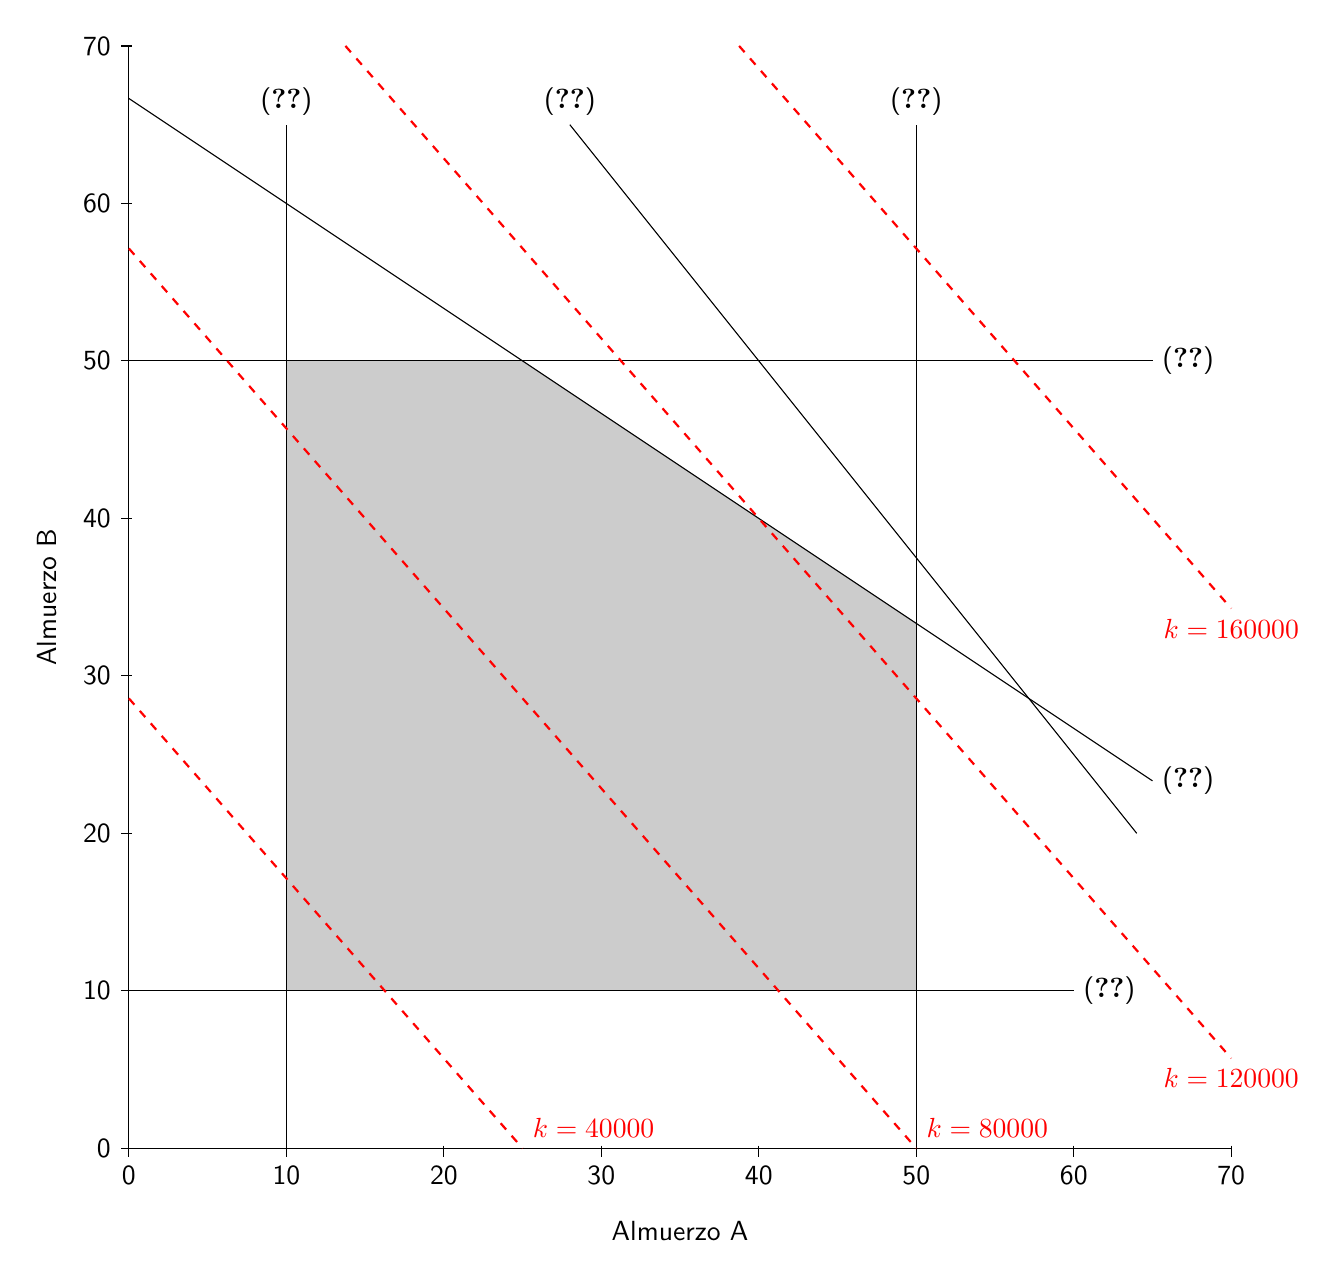
\begin{tikzpicture}[y=.2cm, x=.2cm,font=\sffamily]
		%ejes
		\draw (0,0) -- coordinate (x axis mid) (70,0);
		\draw (0,0) -- coordinate (y axis mid) (0,70);
		%inter
		\foreach \x in {0,10,...,70}
			\draw (\x,1pt) -- (\x,-3pt)
			node[anchor=north] {\x};

		\foreach \y in {0,10,...,70}
			\draw (1pt,\y) -- (-3pt,\y) 
			node[anchor=east] {\y}; 
		%label
		\node[below=0.8cm] at (x axis mid) {Almuerzo A};
		\node[rotate=90, above=0.8cm] at (y axis mid) {Almuerzo B};
		%area
		\fill[gray!40] 
			(10, 10) --
			(10, 50) --
			(25, 50) -- 
			(50, 33.33) --
			(50, 10) -- cycle;
		%lineas
		\draw (10,00) -- (10,65) node[above] {(\ref{1:5})};
		\draw (00,10) -- (60,10) node[right] {(\ref{1:6})};
		\draw (00,50) -- (65,50) node[right] {(\ref{1:4})};
		\draw (50,00) -- (50,65) node[above] {(\ref{1:3})};
		\draw (64,20) -- (28,65) node[above] {(\ref{1:1})};
		\draw (00,66.6666) -- (65,23.3333) node[right] {(\ref{1:2})};
		%f. obj
		\draw[red,thick,dashed]
			(00, 28.57) -- (25, 00) node[above right] {$k=40000$};
		\draw[red,thick,dashed]
			(00, 57.14) -- (50, 00) node[above right] {$k=80000$};
		\draw[red,thick,dashed] 
			(13.75, 70) -- (70, 5.714) node[below] {$k=120000$};
		\draw[red,thick,dashed] 
			(38.75, 70) -- (70, 34.28) node[below] {$k=160000$};
	\end{tikzpicture}
\end{center}

			En el gráfico vemos representadas las restricciones como las rectas,
			la región factible está pintada gris y por ultimo tenemos con lineas
			punteadas algunos valores de la función objetivo.\\
			Del análisis del gráfico vemos como claramente el punto intercepción
			entre la recta (\ref{1:3}) y la recta (\ref{1:2}) es el punto optimo
			en maximización, además, de este mismo análisis podemos concluir que 
			las demás restricciones (\ref{1:1}, \ref{1:4}, \ref{1:5}, \ref{1:6})
			son no-activas.\\
			Cabe destacar que el punto máximo en nuestro gráfico no es entero,
			por lo que, debido a la naturaleza de las variables, debemos buscar
			el entero más cercano a éste que sea máximo. En este caso tenemos
			que el punto optimo es $(50, 33.3)$, los candidatos a máximo serán:
			$(50,33)$ y $(49,34)$ ya que cumplen todas las restricciones. De 
			estos últimos tenemos que el máximo es para $A=49$ y $B=34$ con un
			valor de \$$123000$.
	\end{enumerate}
	\newpage
\section{Pregunta 2}
	\begin{enumerate}
		\item
			\textbf{Buscando función objetivo:} Las variables que modificarán
			nuestras ganancias son:
			\begin{enumerate}
				\item
					\textbf{Smart Fortwo ED importados} ($x_{ed}$) a un costo
					de \$18.000.000 cada uno.
				\item
					\textbf{Volkswagen e-up! importados} ($x_{up}$) a un
					costo de \$23.000.000 cada uno.
				\item
					\textbf{Smart Fortwo ED vendidos} ($y_{ed}$) a 
					\$22.000.000 menos la comisión para el vendedor de 
					\$2.200.000. Ganancia total de \$19.800.000.
				\item
					\textbf{Volkswagen e-up!} ($y_{up}$) a un costo de
					\$30.000.000 menos el 10\% para el vendedor que equivale a
					\$3.000.000. Ganancia total de \$2.700.000.
				\item
					\textbf{Los empleados} (\texttt{T}) a los que debemos pagar
					un sueldo de \$1.200.000 mensual, sin contar su comisión por
					venta.
			\end{enumerate}
			Luego la función objetivo será:
			$$ \textbf{F.O.:} \quad
				\max{Z} = 19800000 \cdot y_{ed} + 
						  27000000 \cdot y_{up} - 
						  18000000 \cdot x_{ed} - 
						  23000000 \cdot x_{up} - 
						  1200000 \cdot \texttt{T} $$
		\item 
			\textbf{Analisando restricciones:} Del texto podemos extraer las
			siguientes restricciones: 
			\begin{align}
				\hspace{4cm}
				x_{ed} &\geq 20 &\emph{(Importar al menos 20 ED)} 
				\label{2:1}\\
				x_{ed} - y_{ed} &\geq 3 &\emph{(Dejar al menos 3 ED
				para exhibir)} \label{2:2}\\
				x_{up} - y_{up} &\geq 3 &\emph{(Dejar al menos 3 UP
				para exhibir)} \label{2:3}\\
				y_{ed} - 0.6 \cdot x_{ed} &\geq 0 &\emph{(Vender al
				menos el 60\% de los ED)} \label{2:4}\\
				y_{up} - 0.6 \cdot x_{up} &\geq 0 &\emph{(Vender al
				menos el 60\% de los UP)} \label{2:5}\\
				0.2 \cdot x_{ed} + 0.2 \cdot x_{up} &= \texttt{T}
				&\emph{(Contratar 1 empleado cada 5 autos)} \label{2:6}\\
				\texttt{T} &\leq 40 &\emph{(Contratar a los más a 40 empleados)}
				\label{2:7}
			\end{align}
			Estas restricciones son las que utilizamos en el código (ver el 
			anexo: sección~\ref{sec:anexo}), el resultado obtenido se muestra
			a continuación, pero para hacer el tableau podemos reducir un poco
			el problema.
			\begin{verbatim}
				Value of objective function: 567600000.00000048
				Actual values of the variables:
				v_ed                           17
				v_up                          177
				i_ed                           20
				i_up                          180
				t                              40
			\end{verbatim}
			Teniendo en cuenta que es una maximización las restricciones 
			(\ref{2:4}) y (\ref{2:5}) pueden ser obviadas, además de de la unión
			de (\ref{2:6}) y (\ref{2:7}) podemos obtener la siguiente
			restricción que incluye ambas:
			\begin{equation} 
				\label{2:8}
				x_{ed} + x_{up} \leq 200
			\end{equation}
		\item
			\textbf{Normalizando las ecuaciones:} Ahora debemos normalizar las
			restricciones (\ref{2:1}), (\ref{2:2}), (\ref{2:3}) y (\ref{2:8}),
			definir la función objetivo y luego construir el tableau.
			\begin{align*}
				\textbf{F.O.:} \quad
				\max{Z} = 19800000  y_{ed} + 
						  27000000  y_{up} - 
						  18240000  x_{ed} - 
						  23240000  x_{up} +
						  0s_1 + \sum_{i=1}^{4} 0s_i -Ma_i
			\end{align*}
			\vspace{-1cm}
			\begin{align*}
				\textbf{S.T.:} \hspace{2cm}
				x_{ed} + x_{up} + s_1&= 200 \\
				x_{up} - y_{up} - e_2 + a_2 &= 3 \\
				x_{ed} - y_{ed} - e_3 + a_3 &= 3 \\
				x_{ed} - e_4 + a_4 &= 20
			\end{align*}
		\item
			\textbf{Resolución por Tableau:}\\
			\textbf{Nota:} Para simplificar la escritura escribiremos los
			millones como unidad, es decir: $1000000 \rightarrow 1$
	\end{enumerate}
	\newpage

	\begin{landscape}
		\vspace*{\fill}
			\begin{itemize}
				\item \textbf{1º iteración}
					\input{tablas/tabla1}\\
					Sale $a_3$ y entra $x_{ed}$.\\
					Realizamos las operaciones fila correspondientes: 
					$f_3\cdot(-1) + f_1$ y $f_3\cdot(-1) + f_4$
				\item \textbf{2º itearación}
					\begin{table}[ht]
	\centering
        \begin{tabular}{ cc|ccccccccccc|cc }
        	& & $y_{ed}$ & $y_{up}$ & $x_{ed}$ & $x_{up}$ & $s_1$ & $e_2$ & $a_2$ & $e_3$ & $a_3$ & $e_4$ & $a_4$ & &\\
        	Base & $c_j$ & 19.8 & 27 & -18.24 & -23.24 & 0 & 0 & -M & 0 & -M & 0 & -M & $b_i$ & $\frac{b_i}{a_{ij}}$\\
        	\hline
                $s_1$    & 0      & 1  & 0  & 0  & 1  & 1  & 0  & 0  & 1  & -1  & 0  & 0  & 197 & 197      \\
                $a_2$    & -M     & 0  & -1 & 0  & 1  & 0  & -1 & 1  & 0  & 0   & 0  & 0  & 3   & -        \\
                $x_{ed}$ & -18.24 & -1 & 0  & 1  & 0  & 0  & 0  & 0  & -1 & 1   & 0  & 0  & 3   & -        \\
                $a_4$    & -M     & 1  & 0  & 0  & 0  & 0  & 0  & 0  & 1  & -1  & -1 & 1  & 17  & \rojo{17}\\
                \hline
                & $z_j$       & 18.24-M & M    & -18.24 & -M & 0 & M & -M & 18.24-M & 18.24+M & M & -M & -54.72-20M & \\ 
                & $c_j - z_j$ & \rojo{1.56+M}  & 27-M & 0 & -23.24+M & 0 & -M & 0 & -18.24+M & 18.24-2M & -M & 0 & &\\ 
        \end{tabular}
\end{table}
\\
					Sale $a_4$ y entra $y_{ed}$.\\
					Realizamos las operaciones fila correspondientes: 
					$f_4\cdot(-1) + f_1$ y $f_4\cdot{1} + f_3$
				\item \textbf{3º itearación}
					\begin{table}[ht]
	\centering
        \begin{tabular}{ cc|ccccccccccc|cc }
        	& & $y_{ed}$ & $y_{up}$ & $x_{ed}$ & $x_{up}$ & $s_1$ & $e_2$ & $a_2$ & $e_3$ & $a_3$ & $e_4$ & $a_4$ & &\\
        	Base & $c_j$ & 19.8 & 27 & -18.24 & -23.24 & 0 & 0 & -M & 0 & -M & 0 & -M & $b_i$ & $\frac{b_i}{a_{ij}}$\\
        	\hline
                $s_1$    & 0      & 0  & 0  & 0  & 1  & 1  & 0  & 0  & 0  & 0   & 1  & -1  & 180 & 180      \\
                $a_2$    & -M     & 0  & -1 & 0  & 1  & 0  & -1 & 1  & 0  & 0   & 0  & 0   & 3   & \rojo{3} \\
                $x_{ed}$ & -18.24 & 0  & 0  & 1  & 0  & 0  & 0  & 0  & 0  & 0   & -1 & 1   & 20  & -        \\
                $y_{ed}$ & 19.8   & 1  & 0  & 0  & 0  & 0  & 0  & 0  & 1  & -1  & -1 & 1   & 17  & -        \\
                \hline
                & $z_j$       & 19.8 & M    & -18.24 & -M & 0 & M & -M & 19.8 & -19.8 & -1.56 & 1.56 & -28.2-3M & \\ 
                & $c_j - z_j$ & 0  & 27-M & 0 & \rojo{-23.24+M} & 0 & -M & 0 & -19.8 & -M+19.8 & 1.56 & -M-1.56 & &\\ 
        \end{tabular}
\end{table}
\\
					Sale $a_2$ y entra $x_{up}$.\\
					Realizamos las operaciones fila correspondientes:
					$f_2\cdot(-1) + f_1$
			\end{itemize}
		\vspace*{\fill}
		\newpage

		\vspace*{\fill}
			\begin{itemize}
				\item \textbf{4º itearación}
					\input{tablas/tabla4}\\
					Sale $s_1$ y entra $y_{up}$.\\
					Realizamos las operaciones fila correspondientes:
					$f_1\cdot{1} + f_2$
				\item \textbf{5º itearación}
					\begin{table}[ht]
	\centering
        \begin{tabular}{ cc|ccccccccccc|cc }
        	& & $y_{ed}$ & $y_{up}$ & $x_{ed}$ & $x_{up}$ & $s_1$ & $e_2$ & $a_2$ & $e_3$ & $a_3$ & $e_4$ & $a_4$ & &\\
        	Base & $c_j$ & 19.8 & 27 & -18.24 & -23.24 & 0 & 0 & -M & 0 & -M & 0 & -M & $b_i$ & $\frac{b_i}{a_{ij}}$\\
        	\hline
                $y_{up}$ & 27     & 0  & 1  & 0  & 0  & 1  & 1  & -1 & 0  & 0   & 1  & -1  & 177 & -         \\
                $x_{up}$ & -23.24 & 0  & 0  & 0  & 1  & 1  & 0  & 0  & 0  & 0   & 1  & -1  & 180 & -         \\
                $x_{ed}$ & -18.24 & 0  & 0  & 1  & 0  & 0  & 0  & 0  & 0  & 0   & -1 & 1   & 20  & -         \\
                $y_{ed}$ & 19.8   & 1  & 0  & 0  & 0  & 0  & 0  & 0  & 1  & -1  & -1 & 1   & 17  & -         \\
                \hline
                & $z_j$       & 19.8 & 27    & -18.24 & -23.24 & 3.76 & 27 & -27 & 19.8 & -19.8 & 2.2 & -2.2 & 537.6 & \\ 
                & $c_j - z_j$ & 0  & 0 & 0 & 0 & -3.76 & -27 & -M-27 & -19.8 & -M+19.8 & -2.2 & -M+2.2 & &\\ 
        \end{tabular}
\end{table}
\\
					Vemos que todos los costos de oportunidad o precios sombras
					son negativos o 0, por tanto estamos en un vértice óptimo,
					con lo que la función objetivo es: 537600000.
					Las diferencias con LPsolve son mínimas, lo que se debe a la
					precisión de cálculo del software, en términos prácticos,
					obtuvimos el mismo resultado, pues los valores de las 
					variables son los mismos.
			\end{itemize}
		\vspace*{\fill}
	\end{landscape}

	\newpage
\section{Pregunta 3}
	Primero, normalizaremos el modelamiento:
\begin{align*}
\textbf{F.O.:} \quad \max z &= 25{x_1} + 15{x_2} + 16{x_3} + 0{s_1} + 0{s_3} + 0{s_4} - M{a_2}
\end{align*}
\vspace{-1cm}
\begin{align*}
	\textbf{S.T.:} \quad
		4{x_2} + 8{x_3} + s_1 &= 1600\\
		10{x_1} + 2{x_2} + a_2 &= 2100\\ 
		x_3 + s_3 &= 300\\ 
		x_2 + s_4 &= 250
\end{align*}

\begin{enumerate}
	\item
		Como $x_2 = 250$ y $x_3 = 75$, tenemos para la restricción 1:
		\begin{align*}
			\hspace{4cm}
				4\cdot250 + 8\cdot75 + s_1 &= 1600 \\ 
				1600 + s_1 &= 1600 \\
				s_1 &= 0
		\end{align*}
		Por lo tanto, $s_1$ no es basal, se ocupan todos los 
		recursos en la restricción 1.

	\item 
		Modificando el coeficiente de $x_2$ en el tableau:
		%%%Tableau
		\begin{table}[ht]
			\centering
			\begin{tabular}{ cc|ccccccc|c }
				& & $x_1$ & $x_2$ & $x_3$ & $s_1$ & $a_2$ & $s_3$ & $s_4$ &\\ 
				Base & $c_j$ & 25 & $15 + \delta$ & 16 & 0 & -M & 0 & 0 & $b_j$ \\
				\hline
				$x_3$ & 16 & 0 & 0 & 1 & 1/8 & 0 & 0 & -1/2 & 75 \\ 
				$x_1$ & 25 & 1 & 0 & 0 & 0 & 1/10 & 0 & -1/5 & 160 \\
				$s_3$ & 0  & 0 & 0 & 0 & -1/8 & 0 & 1 & 1/2 & 225 \\
				$x_2$ & $15 + \delta$ & 0 & 1 & 0 & 0 & 0 & 0 & 1 & 250 \\
				\hline
				& $z_j$ & 25 & $15 + \delta$ & 16 & 2 & 5/2 & 0 & $2 + \delta$ &  \\ 
				& $c_j - z_j$ & 0 & 0 & 0 & -2 & -M-5/2 & 0 & $-2-\delta$ & \\ 
			  \end{tabular}
		\end{table}
		\\Luego el rango de insignificancia para $x_2$ es:
		\begin{align*}
			\hspace{5.33cm}
				-2-\delta &\leq 0  	\quad\emph{(caso max en el que no seguimos iterando)}.\\
				-\delta &\leq 2 \\
				\delta &\geq -2 \\ 
				+\infty &\geq \delta \geq -2 	\quad\emph{(rango de insignificancia)}.
		\end{align*}
		Si el coeficiente de $x_2$ cambia a 10:
		\begin{align*}
			\hspace{5.33cm}
				\Delta{c_j} &= c_j' - c_j \\
			  	\Delta{c_j} &= 10 - 15 \\ 
			  	\Delta{c_j} &= -5 = \delta
		\end{align*}
	  	$-5$ está fuera del rango de insignificancia, por tanto: $-2 - \delta = -2 + 5 = 3 \geq 0$.
		\\Es decir, $s_4$ entra a la base, calculando los $b_j/a_{ij}:$
		\begin{table}[ht]
			\centering
			\begin{tabular}{ cc|cc }
				... & $s_4$ & & \\
				... & 0& $b_j$ & $b_j/a_{ij} $\\
				\hline
				... & -1/2 & 75 & -\\
				... & -1/5 & 160 & - \\
				... & 1/2 & 225 & \textcolor{red}{225/2} \\
				... & 1 & 250 & 250 \\
				\hline
				... & -3 & & \\
				... & 3 & & \\
			\end{tabular}
		\end{table}
		\\Por lo tanto, cambia nuestro óptimo (se debe volver a iterar) y la restricción 3 se vuelve limitante
		(se sale de la base, por lo tanto vale 0 lo que quiere decir que se usan todos los recursos en dicha
		restricción.)
	\item
		\begin{itemize}
			\item 
				\textbf{No activa:} Significa variable artificial $\neq 0$ o
				que está en la base: $s_3 = 225 \Rightarrow$ Restricción 3 es
				inactiva.
			\item 
				\textbf{Activa:} Caso contrario al anterior, restricciones 1,2 
				y 4 no están en base por ende sus variables artificiales son 0,
				por ello son restricciones activas.
		\end{itemize}
	\item Tenemos que:
		\begin{align*}
			%%matriz
			\left[{
				\begin{array}{c}
					Nueva\\
					\\
					soluci\acute{o}n\\			
				\end{array} 
			} \right] 
			=
			\left[{
				\begin{array}{c}
					Soluci\acute{o}n\\
					\\
					actual\\
				\end{array} 
			} \right] 
			+
			\Delta{b_i}a_{ij} \geq 0
		\end{align*}
		Reemplazando por los valores correspondientes a la solución actual y a
		los coeficientes de la variable artificial correspondiente a la
		restricción 1 y naturaleza de las variables, encontraremos el rango para
		$\Delta{b_i}$:.
		\begin{align*}
			\hspace{5.33cm}
				\left[{
					\begin{array}{c}
						75\\
						160\\
						225\\
						250	
					\end{array} 
				} \right] 
				+
				\Delta{b_1}
				\left[{
					\begin{array}{c}
						1/8\\
						0\\
						-1/8\\
						0	
					\end{array} 
				} \right]  
				\geq 0
		\end{align*}
		Luego, el rango para $b_1$:
		\begin{align*}
			\hspace{4cm}
				75 + \Delta{b_1}/8 &\geq 0 \quad \rightarrow \quad \Delta{b_1} \geq -600\\
				225 - \Delta{b_1}/8 &\geq 0 \quad \rightarrow \quad \Delta{b_1} \leq 1800\\
				-600 &\leq \Delta{b_1} \leq 1800 \quad\emph{(Rango dentro del cual no cambia la base)}
		\end{align*}
		Si la solución varía en +1000:
		\begin{align*}
			%%matriz
			\left[{
				\begin{array}{c}
					Nueva\\
					\\
					soluci\acute{o}n\\			
				\end{array} 
			} \right] 
			=
			\left[{
				\begin{array}{c}
					75\\
					160\\
					225\\
					250
				\end{array} 
			} \right] 
			+
			1000
			\left[{
				\begin{array}{c}
					1/8\\
					0\\
					-1/8\\
					0	
				\end{array} 
			} \right]
			=
			\left[{
				\begin{array}{c}
					75 + 1000/8\\
					160\\
					225 - 1000/8\\
					250	
				\end{array} 
			} \right]
			=
			\left[{
				\begin{array}{cc}
					200 & x_3*\\
					160 & x_1*\\
					100 & s_3*\\
					250 & x_2*	
				\end{array} 
			} \right]
			\quad \emph{Nueva solución}
		\end{align*}
		Evaluando en la \textbf{F.O.}: $25\cdot160 + 15\cdot250 + 16\cdot200 + 0\cdot100 = 10950$\\
		{\medskip}\\
		\textbf{Casos Extremos}
		\begin{description}
			\item[Caso 1] $\Delta{b_1} = -600$\\
				\begin{align*}
					%%sol nueva
					\left[{
						\begin{array}{c}
								Nueva\\
							\\
							soluci\acute{o}n\\			
						\end{array} 
					} \right] 
					=
					%%vieja solución
					\left[{
						\begin{array}{c}
							75\\
							160\\
							225\\
							250
						\end{array} 
					} \right] 
					-
					600
					\left[{
						\begin{array}{c}
							1/8\\
							0\\
							-1/8\\
							0	
						\end{array} 
					} \right]
					=
					%%sol final
					\left[{
						\begin{array}{c}
							75 - 600/8\\
							160\\
							225 + 600/8\\
							250	
						\end{array} 
					} \right]
					=
					\left[{
						\begin{array}{cc}
							0 & x_3*\\
							160 & x_1*\\
							300 & s_3*\\
							250 & x_2*	
						\end{array} 
					} \right]
					\quad \emph{Nueva solución}
				\end{align*}
				En este caso, $x_3$ sale de la base.
				\textbf{F.O.} $z = 25\cdot160 + 15\cdot250 + 16\cdot0 + 0\cdot300 = 7750$
			\item[Caso 2] $\Delta{b_1} = 1800$\\
				\begin{align*}
					%%sol nueva
					\left[{
						\begin{array}{c}
								Nueva\\
							\\
							soluci\acute{o}n\\			
						\end{array} 
					} \right] 
					=
					%%vieja solución
					\left[{
						\begin{array}{c}
							75\\
							160\\
							225\\
							250
						\end{array} 
					} \right] 
					+
					1800			
					\left[{
						\begin{array}{c}
							1/8\\
							0\\
							-1/8\\
							0	
						\end{array} 
					} \right]
					=
					%%sol final
					\left[{
						\begin{array}{c}
							75 + 1800/8\\
							160\\
							225 - 1800/8\\
							250	
						\end{array} 
					} \right]
					=
					\left[{
						\begin{array}{cc}
							300 & x_3*\\
							160 & x_1*\\
							0 & s_3*\\
							250 & x_2*	
						\end{array} 
					} \right]
					\quad \emph{Nueva solución}
				\end{align*}
				En este caso, $s_3$ sale de la base.
				\textbf{F.O.} $z = 25\cdot160 + 15\cdot250 + 16\cdot300 + 0\cdot0 = 12550$
		\end{description}
	\item
		Evaluemos las variables implicadas en la nueva restricción ($x_1 = 160, x_2=250, x_3=75$):
		\begin{align*}
			\hspace{4cm}
				6x_1 + 3x_2 + 4x_3 &\leq 1900\\
				6\cdot160 + 3\cdot250 + 4\cdot75 &= 2010 \geq 1900
		\end{align*}
		Luego, no se cumple la restricción. Para resolver el problema, debemos retroceder en el tableau y chequear la restricción
		hasta que se cumpla, luego volver a iterar hasta hallar la nueva solución.
\end{enumerate}

\section{Conclusiones}
	\begin{itemize}
	\item
		\textbf{Parte 1:} Si bien en un principio el modelo aparenta tener varias
		variables, un análisis adecuado nos permite llegar a las que realmente 
		influyen en el proceso de optimización. Por otra parte, se hacen
		evidentes las limitaciones del método gráfico, si bien su carácteristica
		principal es ser bastante claro al momento de visualizar la región
		factible y las soluciones, cuando el modelo se vuelve más complejo, el
		método se vuelve inútil.
	\item
		\textbf{Parte 2:} Sabemos que hay muchas formas de modelar, por lo mismo
		hay que considerar varias opciones al momento de escoger un modelo. En
		un principio nuestro modelo de optimización era complejo, sin embargo,
		con las debidas modificaciones pudimos simplificar el problema y
		resolver el tableu en menos iteraciones. A esto, el software nos 
		permitió ''jugar'' de manera rápida con las variables y restricciones,
		de manera que pudimos comprobar nuestras sospechas y verificar que el
		modelo era correcto.
	\item
		\textbf{Parte 3:} El análisis de sensibilidad nos permite analizar de
		manera directa los cambios en varias zonas de un modelo, ya sean
		recursos, variables nuevas, restricciones nuevas, etc. Este proceso nos
		permite ahorrar bastante tiempo dado que no es necesario volver a
		resolver el modelo completo. Por otro lado, nos permite tener un control
		más claro, a la hora de tomar decisiones respecto a las variables que
		modifican más nuestras predicciones.
\end{itemize}

\section{Anexo} \label{sec:anexo}
	%hack para acentos:
	\lstset{literate=
		{á}{{\'a}}1 {é}{{\'e}}1 {í}{{\'i}}1 {ó}{{\'o}}1 {ú}{{\'u}}1
		{Á}{{\'A}}1 {É}{{\'E}}1 {Í}{{\'I}}1 {Ó}{{\'O}}1 {Ú}{{\'U}}1
		{à}{{\`a}}1 {è}{{\'e}}1 {ì}{{\`i}}1 {ò}{{\`o}}1 {ù}{{\`u}}1
		{À}{{\`A}}1 {È}{{\'E}}1 {Ì}{{\`I}}1 {Ò}{{\`O}}1 {Ù}{{\`U}}1
		{ä}{{\"a}}1 {ë}{{\"e}}1 {ï}{{\"i}}1 {ö}{{\"o}}1 {ü}{{\"u}}1
		{Ä}{{\"A}}1 {Ë}{{\"E}}1 {Ï}{{\"I}}1 {Ö}{{\"O}}1 {Ü}{{\"U}}1
		{â}{{\^a}}1 {ê}{{\^e}}1 {î}{{\^i}}1 {ô}{{\^o}}1 {û}{{\^u}}1
		{Â}{{\^A}}1 {Ê}{{\^E}}1 {Î}{{\^I}}1 {Ô}{{\^O}}1 {Û}{{\^U}}1
		{œ}{{\oe}}1 {Œ}{{\OE}}1 {æ}{{\ae}}1 {Æ}{{\AE}}1 {ß}{{\ss}}1
		{ç}{{\c c}}1 {Ç}{{\c C}}1 {ø}{{\o}}1 {å}{{\r a}}1 {Å}{{\r A}}1
		{€}{{\EUR}}1 {£}{{\pounds}}1
	}
	%Anexo con código utilizado
	\lstinputlisting[
	             frame=single,
	             showstringspaces=false,
	             commentstyle=\color{gris},
	             title=\lstname,
	             tabsize=4]{pregunta2.lp}
\vfill\hfill HV/AS/\LaTeXe
\end{document}
